\documentclass[preprint, 3p,
authoryear]{elsarticle} %review=doublespace preprint=single 5p=2 column
%%% Begin My package additions %%%%%%%%%%%%%%%%%%%

\usepackage[hyphens]{url}

  \journal{Ecological Entomology} % Sets Journal name

\usepackage{lineno} % add
  \linenumbers % turns line numbering on

\usepackage{graphicx}
%%%%%%%%%%%%%%%% end my additions to header

\usepackage[T1]{fontenc}
\usepackage{lmodern}
\usepackage{amssymb,amsmath}
\usepackage{ifxetex,ifluatex}
\usepackage{fixltx2e} % provides \textsubscript
% use upquote if available, for straight quotes in verbatim environments
\IfFileExists{upquote.sty}{\usepackage{upquote}}{}
\ifnum 0\ifxetex 1\fi\ifluatex 1\fi=0 % if pdftex
  \usepackage[utf8]{inputenc}
\else % if luatex or xelatex
  \usepackage{fontspec}
  \ifxetex
    \usepackage{xltxtra,xunicode}
  \fi
  \defaultfontfeatures{Mapping=tex-text,Scale=MatchLowercase}
  \newcommand{\euro}{€}
\fi
% use microtype if available
\IfFileExists{microtype.sty}{\usepackage{microtype}}{}
\usepackage[]{natbib}
\bibliographystyle{plainnat}

\ifxetex
  \usepackage[setpagesize=false, % page size defined by xetex
              unicode=false, % unicode breaks when used with xetex
              xetex]{hyperref}
\else
  \usepackage[unicode=true]{hyperref}
\fi
\hypersetup{breaklinks=true,
            bookmarks=true,
            pdfauthor={},
            pdftitle={How does tree harvest influence benthic invertebrate density?},
            colorlinks=false,
            urlcolor=blue,
            linkcolor=magenta,
            pdfborder={0 0 0}}

\setcounter{secnumdepth}{5}
% Pandoc toggle for numbering sections (defaults to be off)


% tightlist command for lists without linebreak
\providecommand{\tightlist}{%
  \setlength{\itemsep}{0pt}\setlength{\parskip}{0pt}}



\usepackage{float}



\begin{document}


\begin{frontmatter}

  \title{How does tree harvest influence benthic invertebrate density?}
    \author[McGill University]{Sam Straus%
  \corref{cor1}%
  \fnref{1}}
   \ead{samantha.straus@mcgill.ca} 
    \author[Another University]{Bob Security}
   \ead{bob@example.com} 
    \author[Another University]{Cat Memes%
  %
  \fnref{2}}
   \ead{cat@example.com} 
    \author[Some Institute of Technology]{Derek Zoolander%
  %
  \fnref{2}}
   \ead{derek@example.com} 
      \affiliation[Some Institute of Technology]{Department, Street,
City, State, Zip}
    \affiliation[Another University]{Department, Street, City, State,
Zip}
    \cortext[cor1]{Corresponding author}
  
  \begin{abstract}
  We looked at the density of Baetis spp. in harvested and non-harvested
  stream catchments.
  \end{abstract}
    \begin{keyword}
    stream ecology \sep 
    entomology
  \end{keyword}
  
 \end{frontmatter}

\hypertarget{introduction}{%
\section{Introduction}\label{introduction}}

\emph{Baetis} spp, belonging to the insect order Ephemeroptera, are
commonly used as stream quality indicators \citep{wallace1986response}.

\hypertarget{methods}{%
\section{Methods}\label{methods}}

Researchers collected data on the number of \emph{Baetis} spp. per
square meter in the benthic environment of various catchments from 1995
to 2005. Some of the catchments were harvested, while others were not.

\hypertarget{results}{%
\section{Results}\label{results}}

Figure \ref{fig1} is generated using an R chunk.

\begin{figure}[H]

{\centering 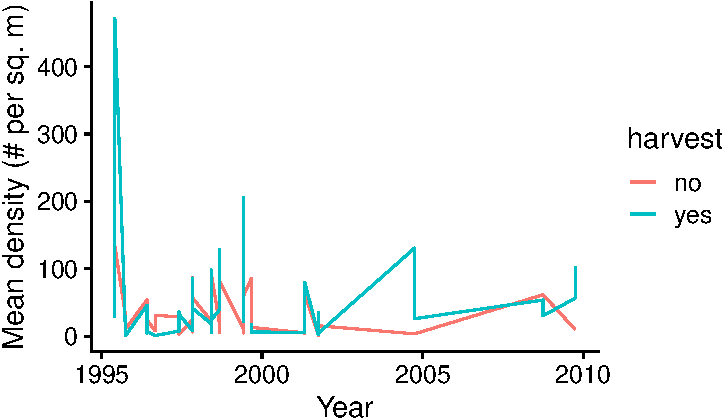
\includegraphics[width=0.75\linewidth]{Assignment_mockarticle_files/figure-latex/fig1-1} 

}

\caption{\label{fig1}Baetis density in harvested and non-harvested catchments}\label{fig:fig1}
\end{figure}

\hypertarget{discussion}{%
\section{Discussion}\label{discussion}}

\emph{Baetis} sp. (Ephemeroptera) are used as stream quality indicators
for catchments \citep{wallace1986response}.

\renewcommand\refname{References}
\bibliography{mybibfile.bib}


\end{document}
